% !TeX root = ../../thesis.tex
\chapter{Manual}\label{ch:manual}




\section{Tips and Tricks}

\subsection{Image on the cover page}

If you want to place an image on the cover of the dissertation, you can add
the code underneath to the template (check with your promotor whether this is
allowed).

\paragraph{Include image:}
Search for the \texttt{\textbackslash frontcoverheaderXII} command in
the \texttt{adsphd.cls} file and add the following lines:
\begin{verbatim}
   \begin{textblock*}{56mm}(10mm+#1,15mm)
   \includegraphics[width=56mm,height=20mm]{image/filename}
   \end{textblock*}
\end{verbatim}
Where 56mm is the width, 20mm the height, 10mm the x-location and 15mm the
y-location.

\paragraph{Change cover font color:}
Add the command \texttt{\textbackslash color\{red\}} to the
\texttt{\textbackslash frontcoverheaderXII} command or enclose specific parts.
For example, \texttt{\{\textbackslash color\{red\}\textbackslash
textbf\{\textbackslash @authorf\textbackslash\ \textbackslash @authorl\}}.

\subsection{Full cover page}

\textbf{Important}: most printing services will create their own cover page based
on the details you send them (title, name, affiliation, ...) and do not supply
you with all necessary parameters (e.g., thickness of the paper) because these
differ from machine to machine. Therefore, the generated cover page is only
indicative and probably not used by your printing server (or even correct).


A full cover page (combining front cover, spine and back cover) can be
generated automatically using the command \texttt{make cover} or \texttt{python3 run.py cover}. This creates a pdf
\texttt{\$(COVERPDF);} by default this is \texttt{cover.pdf}.

The width of the spine is set by redefining \texttt{\\adsphdspinewidth} (9mm by default).

It can be seen in the provided \texttt{thesis.tex} that all information necessary to
generate a cover page is contained between two markers

\begin{verbatim}
    %%% COVER: Settings %%%
    ...
    %%% COVER: End settings %%%
\end{verbatim}

DO NOT REMOVE THESE!! They are used by the Makefile!!

The default front and/or back cover page can be overwritten: 

\begin{itemize}
    \item create a file \texttt{mycoverpage.tex}
    \item redefine the commands \texttt{\textbackslash makefrontcovergeneral} and \texttt{\textbackslash makebackcovergeneral}. For
          an example and more information, see the provided file \texttt{mycoverpage.tex}.
\end{itemize}

The cover page in the generated pdf has the following structure:

{\tiny
\begin{verbatim}
    <--rbleed--><--backcoverpage--><--lbleed--><--spine width--><--lbleed--><--frontcoverpage--><--rbleed-->
\end{verbatim}
}

The default bleed (both lbleed and rbleed) is 7mm. I suggest not changing this
value unless you know what you are doing ;) The latter can be done by
redefining \texttt{\textbackslash defaultlbleed} and \texttt{\textbackslash defaultrbleed} respectively.


\subsection{Table of contents}

To remove list of figures, tables and other preface chapters from the table of
contents, search for occurrences of \texttt{\textbackslash addcontentsline} in the file
\texttt{adsphd.cls} and comment them.

\subsection{Small ebook size}

When you add the \texttt{epub} option to the adsphd class the dissertation is
printed to a smaller size to read on a device such as Kindle.

Environments such as tables or tikZ pictures are often sized in absolute values
and not relative to the size of the output. You can wrap them in a resizebox
to enforce scaling:

\begin{verbatim}
  \resizebox{\textwidth}{!}{%
    \begin{tabular}{cc}
      ...
    \end{tabular}
  }
\end{verbatim}

\section{Settings for TeXstudio}

If you are working with TeXstudio or other windows latex editors you might want to adjust the editor's settings to allow a proper compilation of the table of contents and list of figures/tables.

\subsection{Custom \textit{makeindex} and \textit{makeglossaries} commands}

According to the \textit{README.md} the tables are indexed through two custom commands. To edit them in TeXstudio open the \textit{Commands} settings (\textit{Options $\to$ Configure TeXstudio...,  Commands} sheet), edit the following fields and press OK.

\textit{Makeindex}:
{\scriptsize
\begin{verbatim}
"C:/Program Files/MiKTeX 2.9/miktex/bin/x64/makeindex.exe" %.nlo -s nomencl.ist -o %.nls
\end{verbatim}}

\textit{Makeglossaries}:
{\scriptsize
\begin{verbatim}
"C:/Program Files/MiKTeX 2.9/miktex/bin/x64/makeindex.exe" %.glo -s %.ist -t %.glg -o %.gls
\end{verbatim}}

Now the customized commands can be launched by using \textit{Tools $\to$ Commands $\to$ MakeIndex/Makeglossaries}. If you want to automatize it in the standard \textit{Build \& View} (F5) and \textit{Compile} (F6) commands look at the following section.

\subsection{Custom Build\&View and Compile meta-commands}

Open \textit{Options $\to$ Configure TeXstudio...,  Build} sheet, edit the following field and press OK.

\textit{Build \& View}:
{\footnotesize\begin{verbatim}
	txs:///pdflatex | txs:///bibtex | txs:///makeglossaries | txs:///makeindex |
	txs:///pdflatex  | txs:///pdflatex
	\end{verbatim}}

To view the PDF once created you have to press F7 (or \textit{Tool $\to$ View}) and the PDF will automatically update in the default viewer whan you modify it. 

If you prefer to directly view the created PDF\textbf{ from the beginning }edit the field as follow:
{\footnotesize\begin{verbatim}
	txs:///pdflatex | txs:///bibtex | txs:///makeglossaries | txs:///makeindex |
	txs:///pdflatex  | txs:///pdflatex | txs:///view-pdf
	\end{verbatim}}

\begin{figure}  [htbp]
\captionsetup[subfigure]{justification=centering}
\centering
\begin{subfigure}{.5\textwidth}
  \centering
  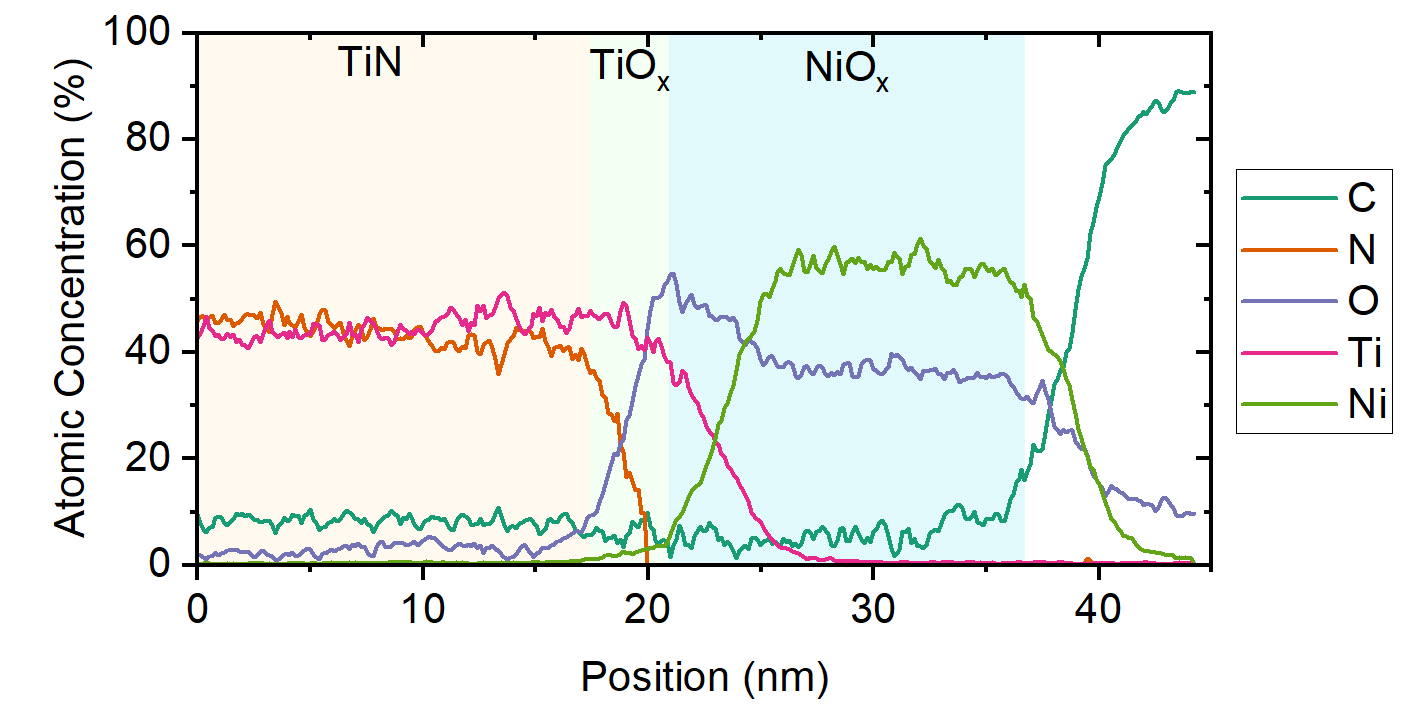
\includegraphics[width=\linewidth]{chapters/manual/image/Sample1.png}
  \caption{$V_{DS} = 49 V$ }

  \label{fig:chipir:IRFR:49}
  \captionsetup{justification=centering}
\end{subfigure}%
\begin{subfigure}{.5\textwidth}
  \centering
  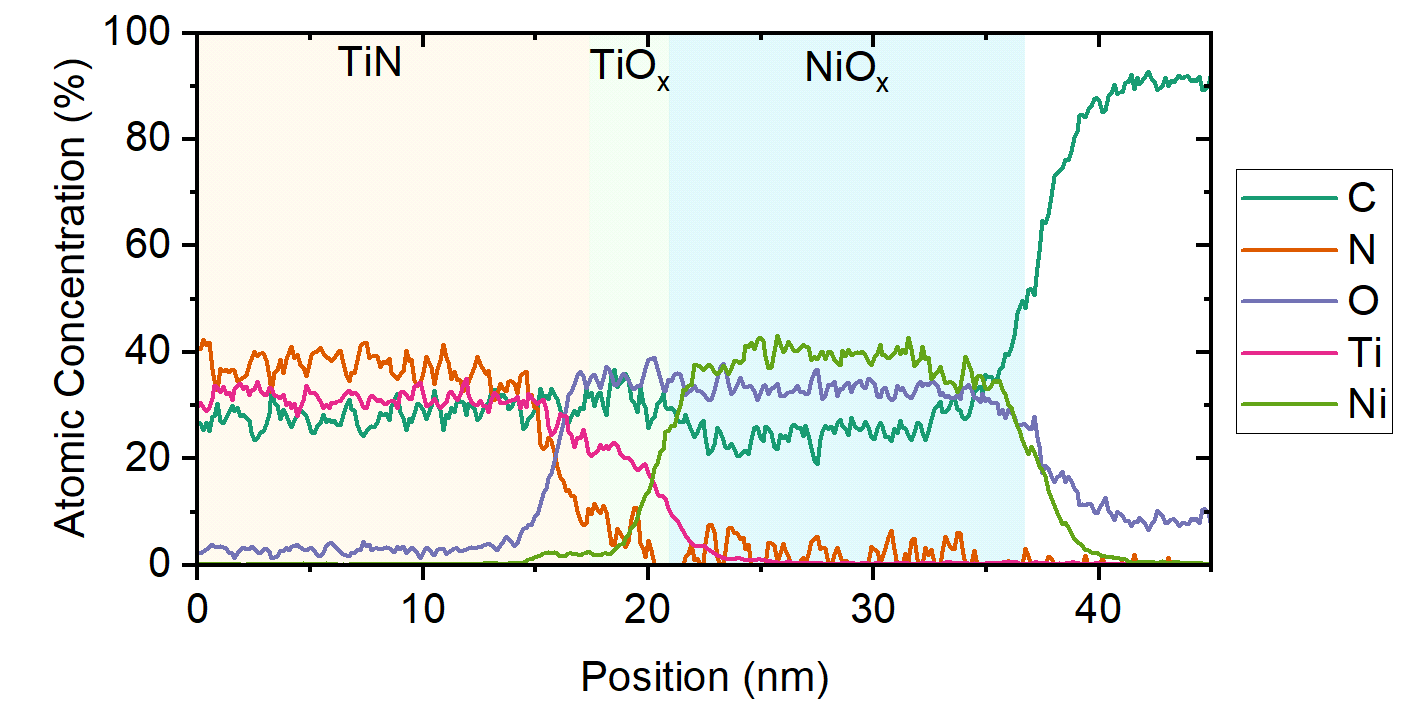
\includegraphics[width=\linewidth]{chapters/manual/image/Sample2.png}
  \caption{$V_{DS} = 50 V$}
  \label{fig:chipir:irfr:50}
\end{subfigure}

\begin{subfigure}{.5\textwidth}
  \centering
  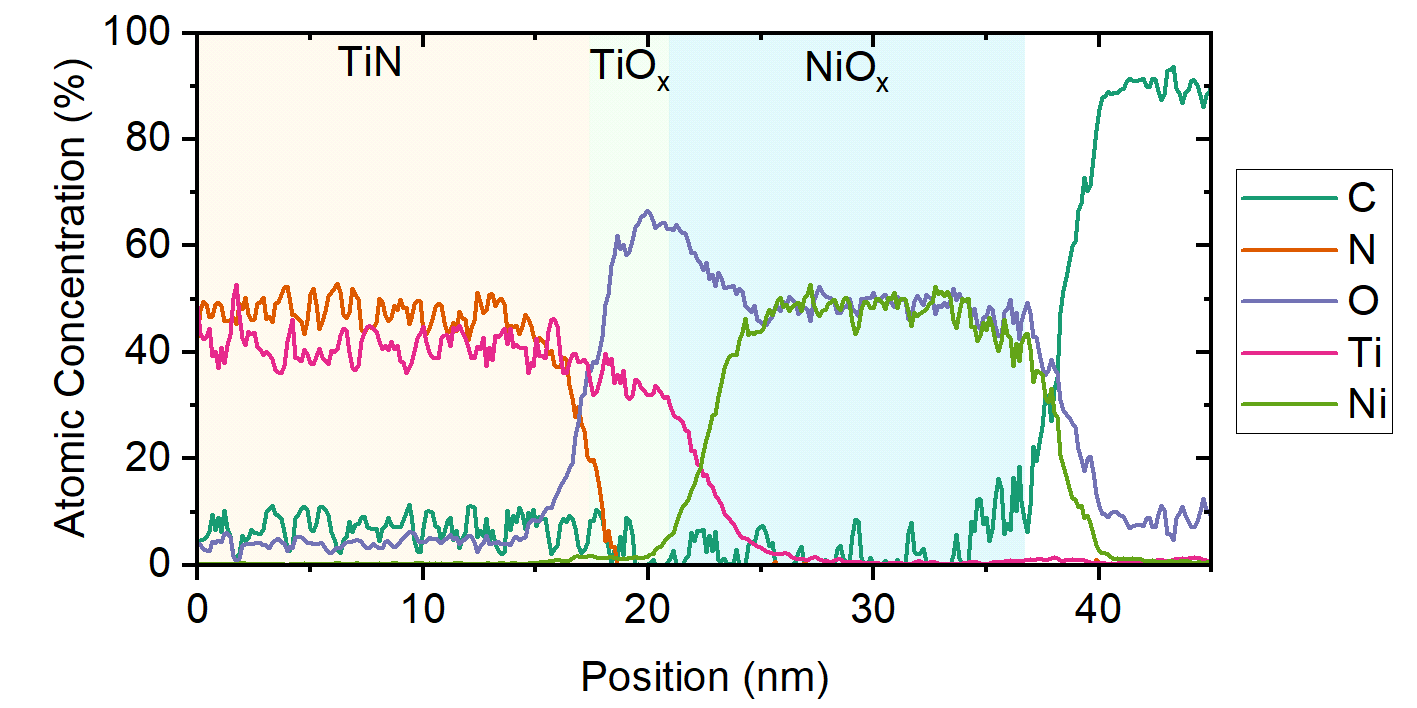
\includegraphics[width=\linewidth]{chapters/manual/image/Sample3.png}
  \caption{$V_{DS} = 52 V$ }

  \label{fig:chipir:irfr:52}
  \captionsetup{justification=centering}
\end{subfigure}%
\begin{subfigure}{.5\textwidth}
  \centering
  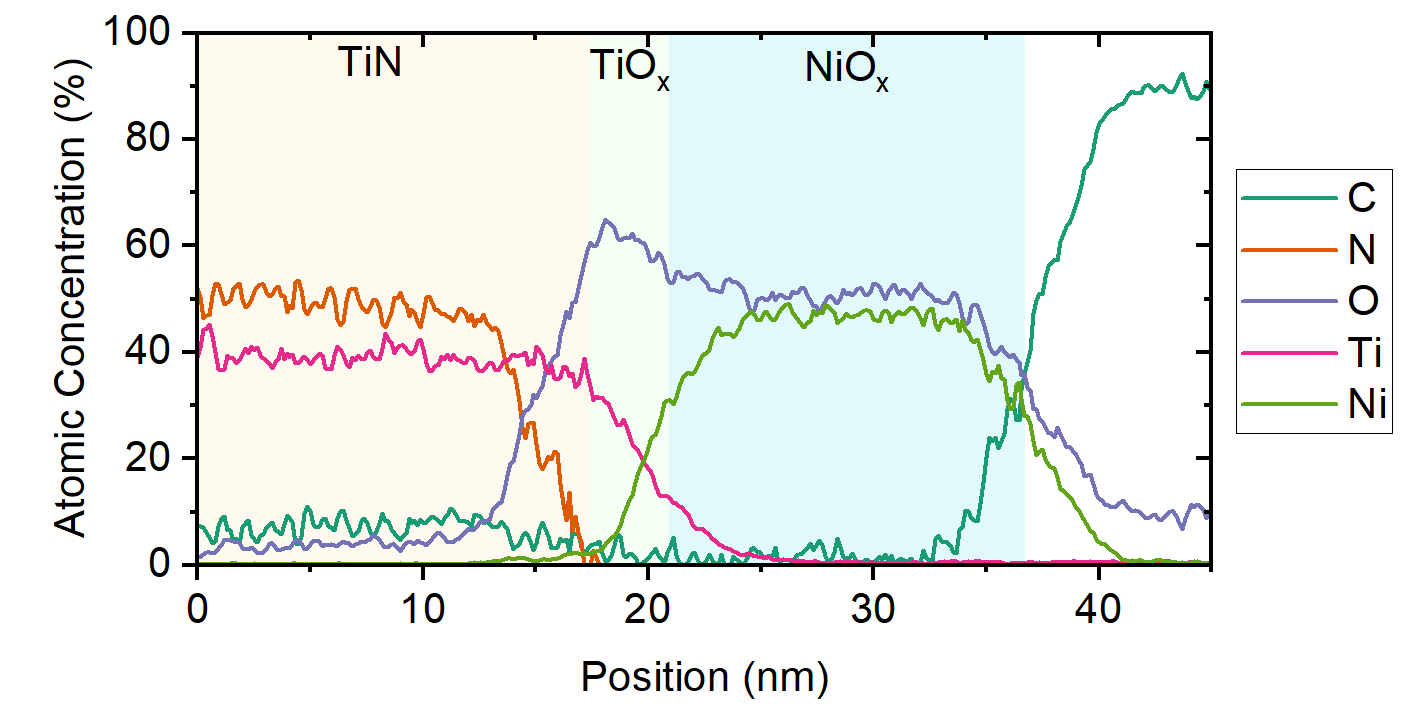
\includegraphics[width=\linewidth]{chapters/manual/image/Sample4.png}
  \caption{$V_{DS} = 54 V$}
  \label{fig:chipir:irfr:54}
\end{subfigure}

\end{figure}




%%%%%%%%%%%%%%%%%%%%%%%%%%%%%%%%%%%%%%%%%%%%%%%%%%
% Keep the following \cleardoublepage at the end of this file, 
% otherwise \includeonly includes empty pages.
\cleardoublepage

